%%%%%%%%%%%%%%%%%%%%%%%%%%%%%%%%%%%%%%%%%%%%%%%%%%%%%%%%%%%%%%%%%%%%%%%%%%%%%
%
%  System        : 
%  Module        : 
%  Object Name   : $RCSfile$
%  Revision      : $Revision$
%  Date          : $Date$
%  Author        : $Author$
%  Created By    : Robert Heller
%  Created       : Wed Nov 16 09:04:20 2022
%  Last Modified : <221116.1227>
%
%  Description 
%
%  Notes
%
%  History
% 
%%%%%%%%%%%%%%%%%%%%%%%%%%%%%%%%%%%%%%%%%%%%%%%%%%%%%%%%%%%%%%%%%%%%%%%%%%%%%
%
%    Copyright (C) 2022  Robert Heller D/B/A Deepwoods Software
%			51 Locke Hill Road
%			Wendell, MA 01379-9728
%
%    This program is free software; you can redistribute it and/or modify
%    it under the terms of the GNU General Public License as published by
%    the Free Software Foundation; either version 2 of the License, or
%    (at your option) any later version.
%
%    This program is distributed in the hope that it will be useful,
%    but WITHOUT ANY WARRANTY; without even the implied warranty of
%    MERCHANTABILITY or FITNESS FOR A PARTICULAR PURPOSE.  See the
%    GNU General Public License for more details.
%
%    You should have received a copy of the GNU General Public License
%    along with this program; if not, write to the Free Software
%    Foundation, Inc., 675 Mass Ave, Cambridge, MA 02139, USA.
%
% 
%
%%%%%%%%%%%%%%%%%%%%%%%%%%%%%%%%%%%%%%%%%%%%%%%%%%%%%%%%%%%%%%%%%%%%%%%%%%%%%

\chapter{PocketBeagleCommandStation: A LCC/DCC Command Station based on a Pocket Beagle}

Through hole version of the PocketBeagle LCC\footnote{Layout Command Control,
See \url{https://www.nmra.org/lcc} for more details and available standards
documentation.}/DCC Command Station. This is a DCC command station that is a
LCC node. It implements the OpenLCB train protocol node over LCC and converts
that to DCC commands. It includes a booster and puts the DCC signal on the LCC
bus (pins 4 and 5). It implements a programming track and implements Railcom.
The Command Station uses a PocketBeagle as the processing element and uses the
PRUs (Programmable Realtime Units) to generate the DCC signal. 

\section{Circuit Description}
 
\subsection{Section Interconnect}
\begin{figure}[hbpt]\begin{centering}%
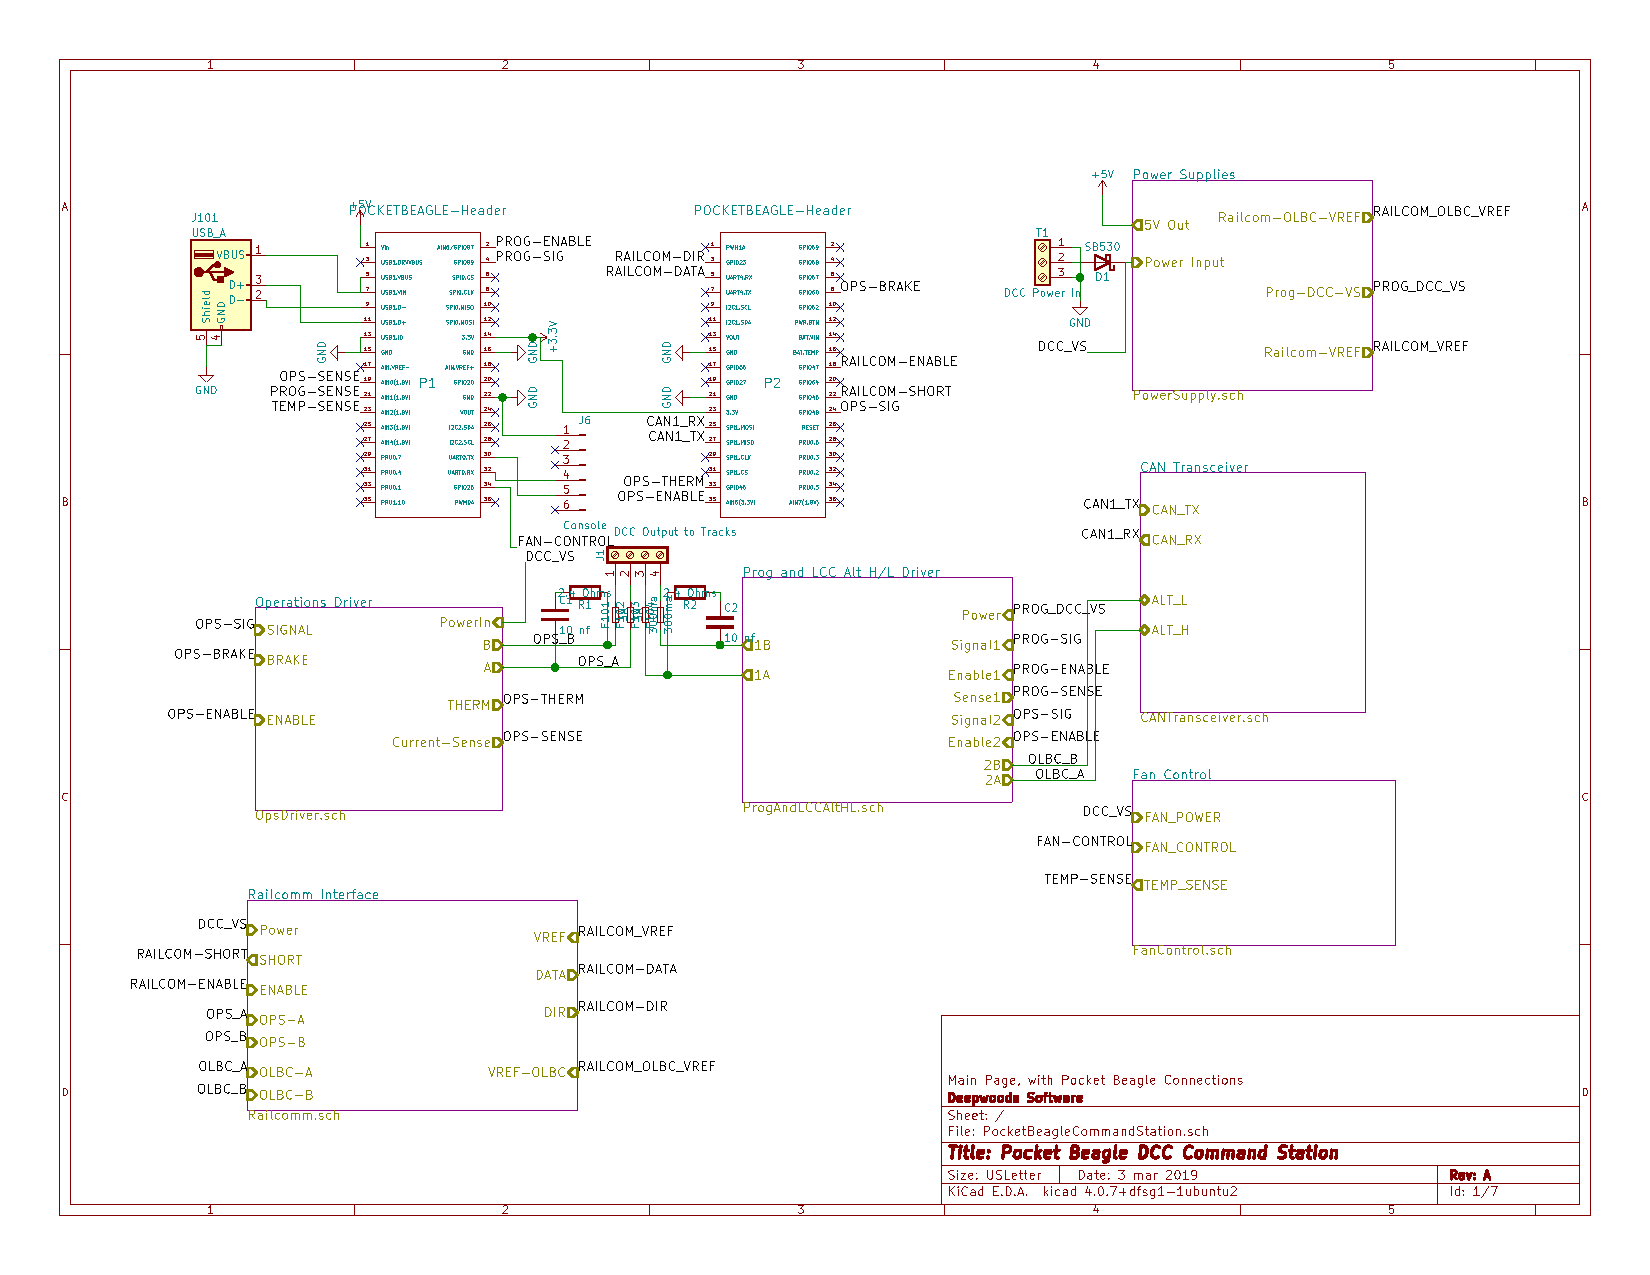
\includegraphics[width=4in]{PocketBeagleCommandStation-1.pdf}
\caption{Circuit Diagram of the PocketBeagleCommandStation board, page 1: Main 
sheet -- Section Interconnect}
\end{centering}\end{figure}
\begin{figure}[hbpt]\begin{centering}%
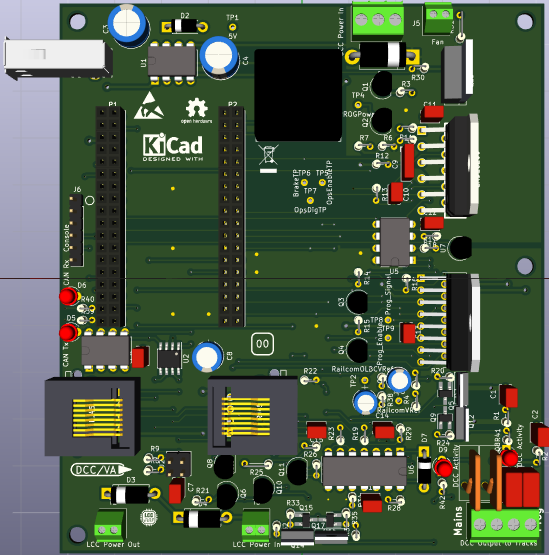
\includegraphics[width=4in]{PocketBeagleCommandStation.png}
\caption{3D Rendering of the whole board.}
\end{centering}\end{figure}

This shows how the various subsections are interconnected.
\clearpage
\subsection{Power Supplies}
\begin{figure}[hbpt]\begin{centering}%
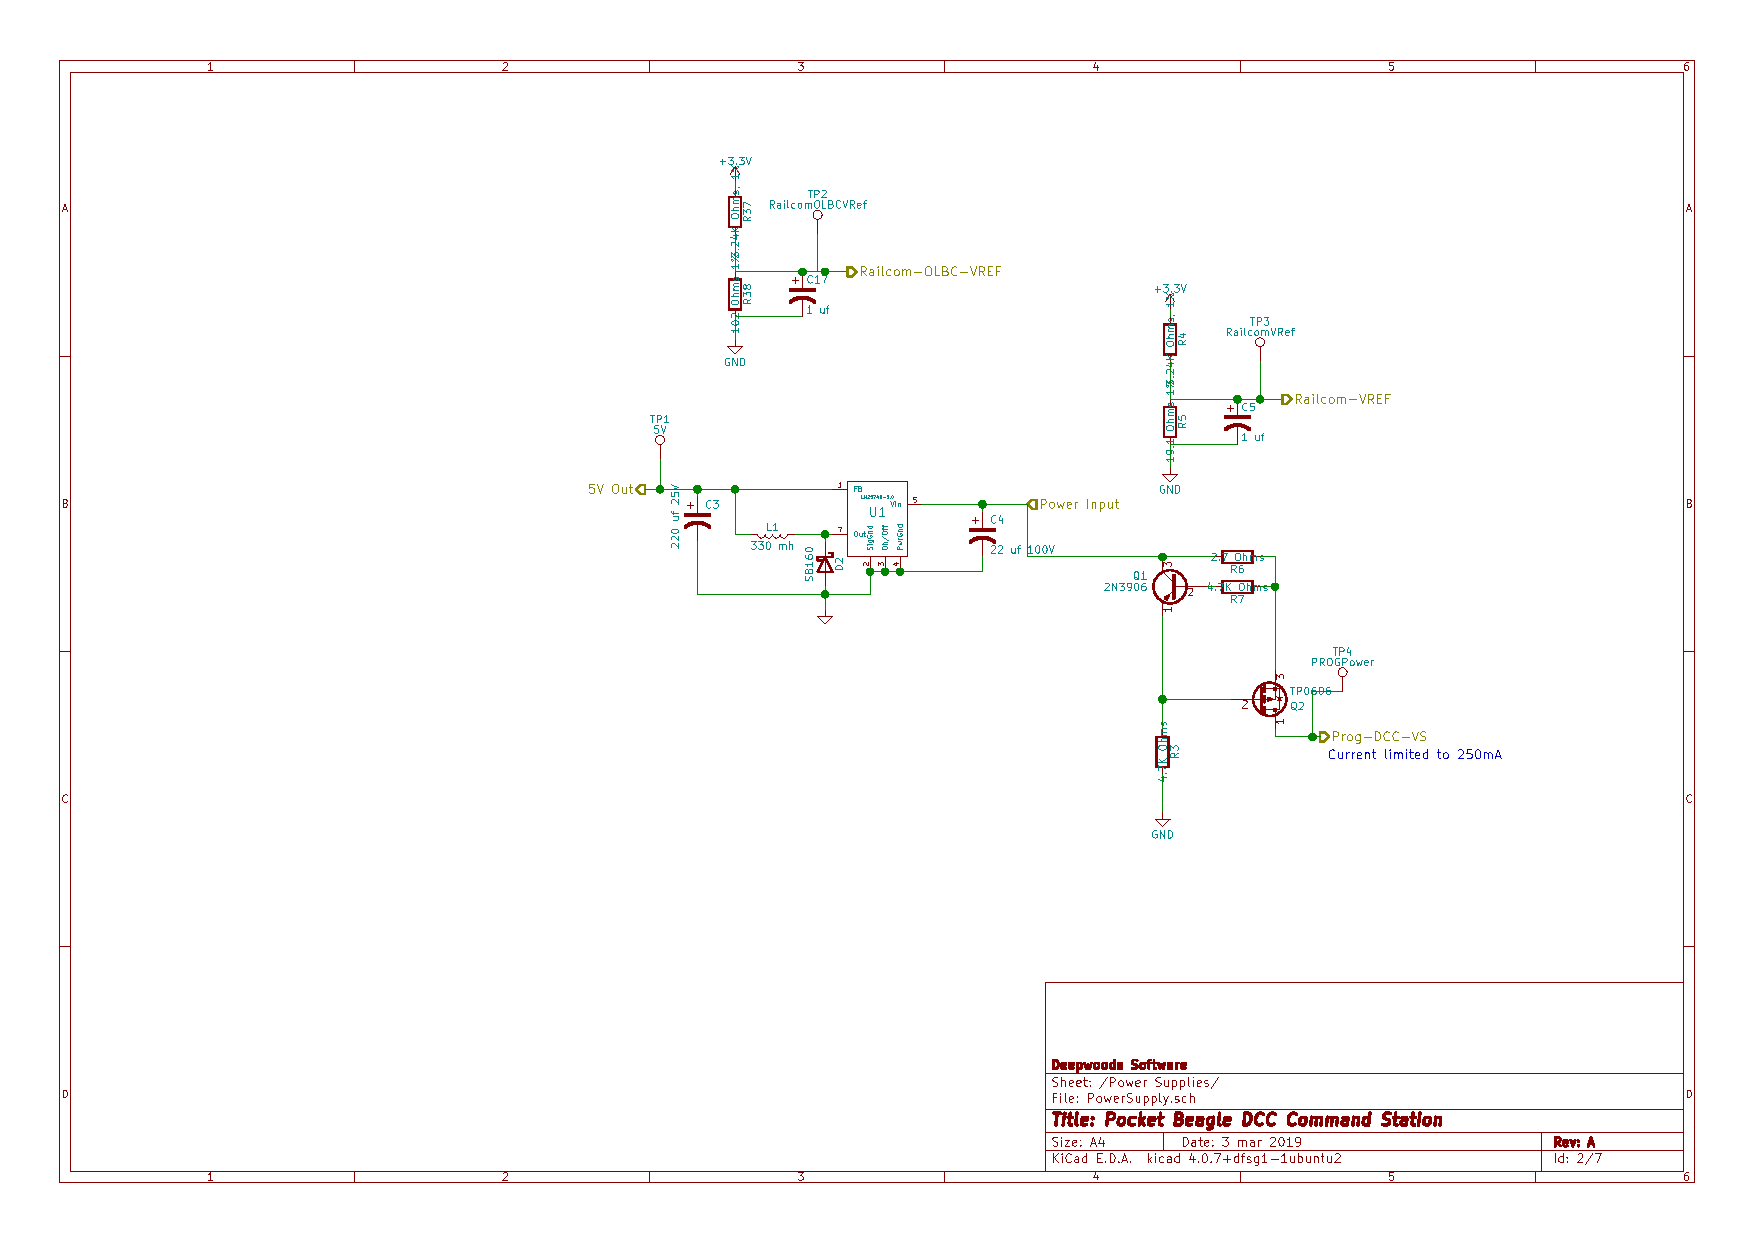
\includegraphics[width=4in]{PocketBeagleCommandStation-2.pdf}
\caption{Circuit Diagram of the PocketBeagleCommandStation board, page 2: 
Power Supplies}
\end{centering}\end{figure} 

This shows the power supply circuits.
\clearpage
\subsection{CAN Transceiver}
\begin{figure}[hbpt]\begin{centering}%
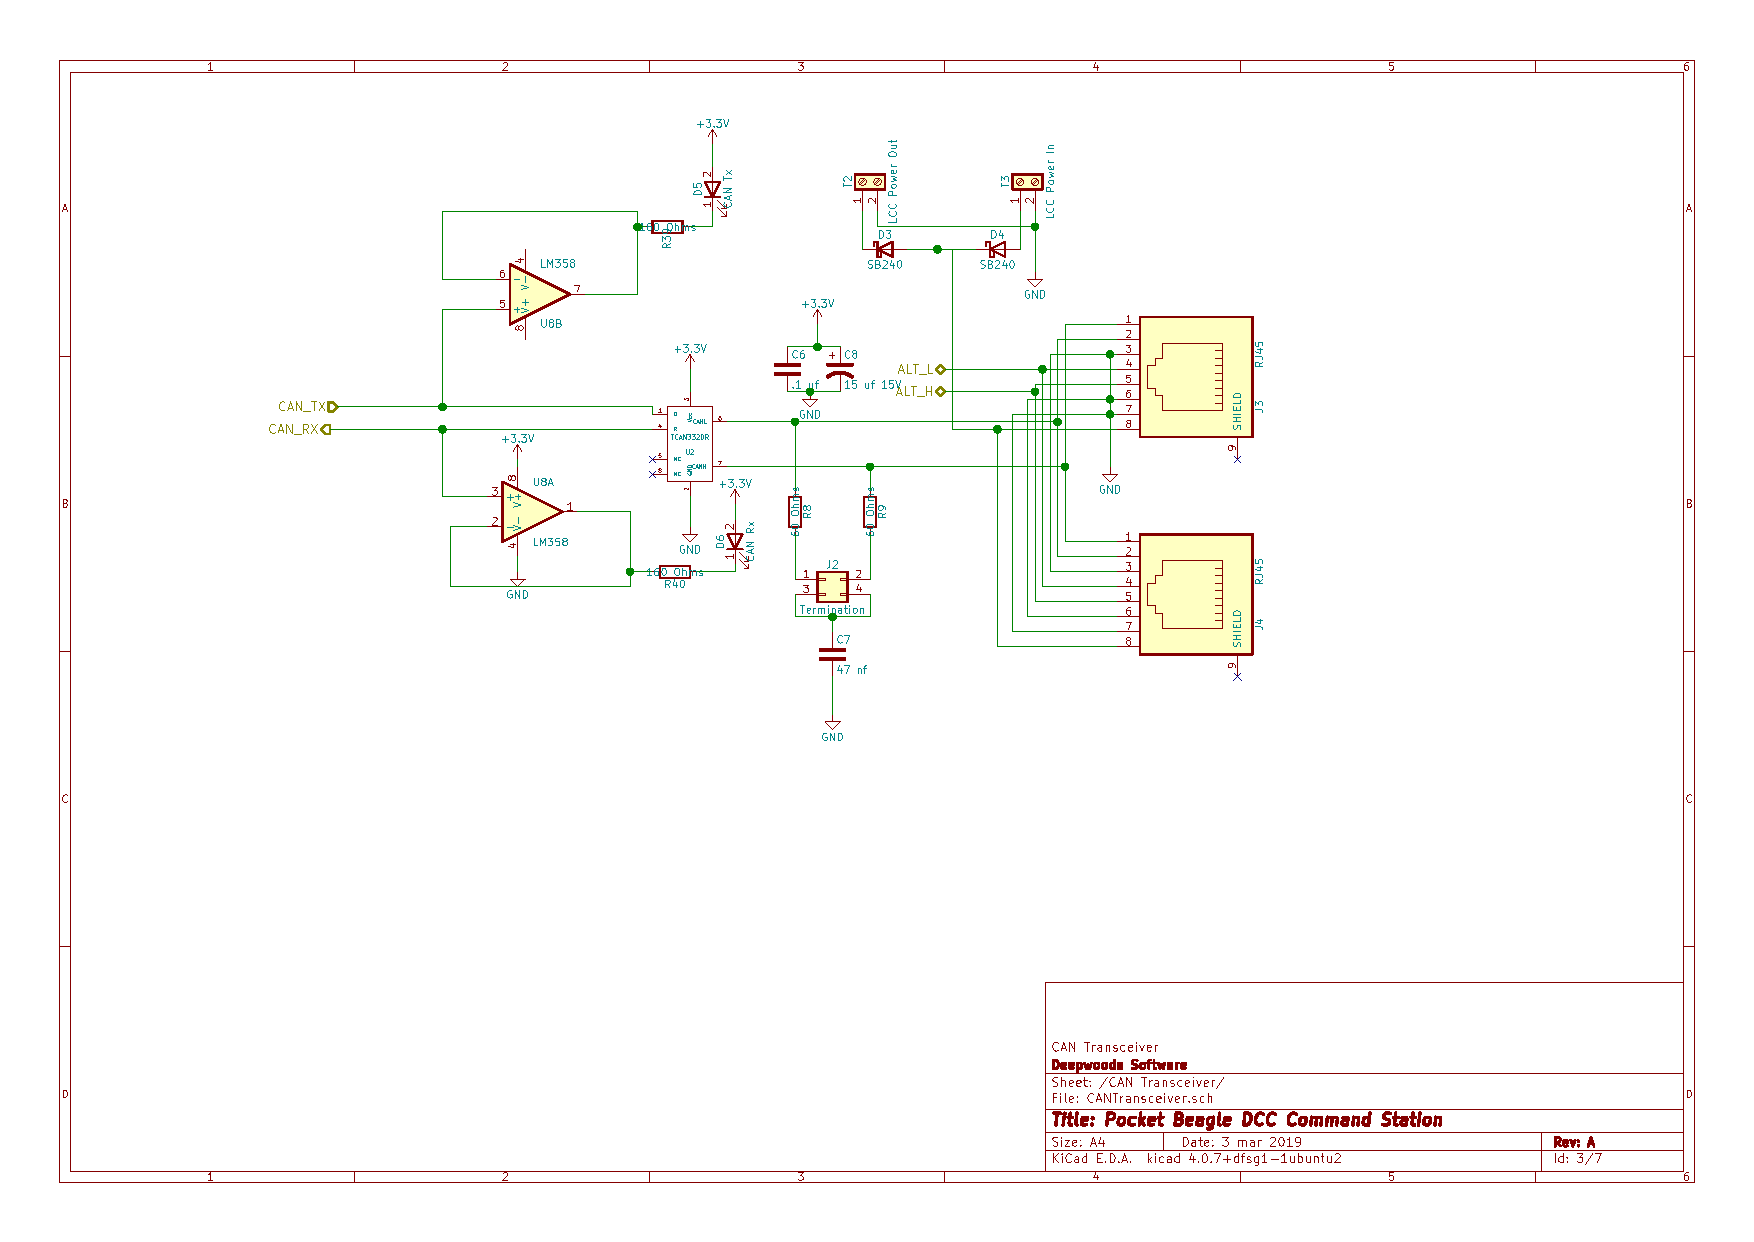
\includegraphics[width=4in]{PocketBeagleCommandStation-3.pdf}
\caption{Circuit Diagram of the PocketBeagleCommandStation board, page 3: CAN 
Transceiver}
\end{centering}\end{figure}

This shows the CAN Transceiver circuitry.
\clearpage
\subsection{OPS DCC Driver}
\begin{figure}[hbpt]\begin{centering}%
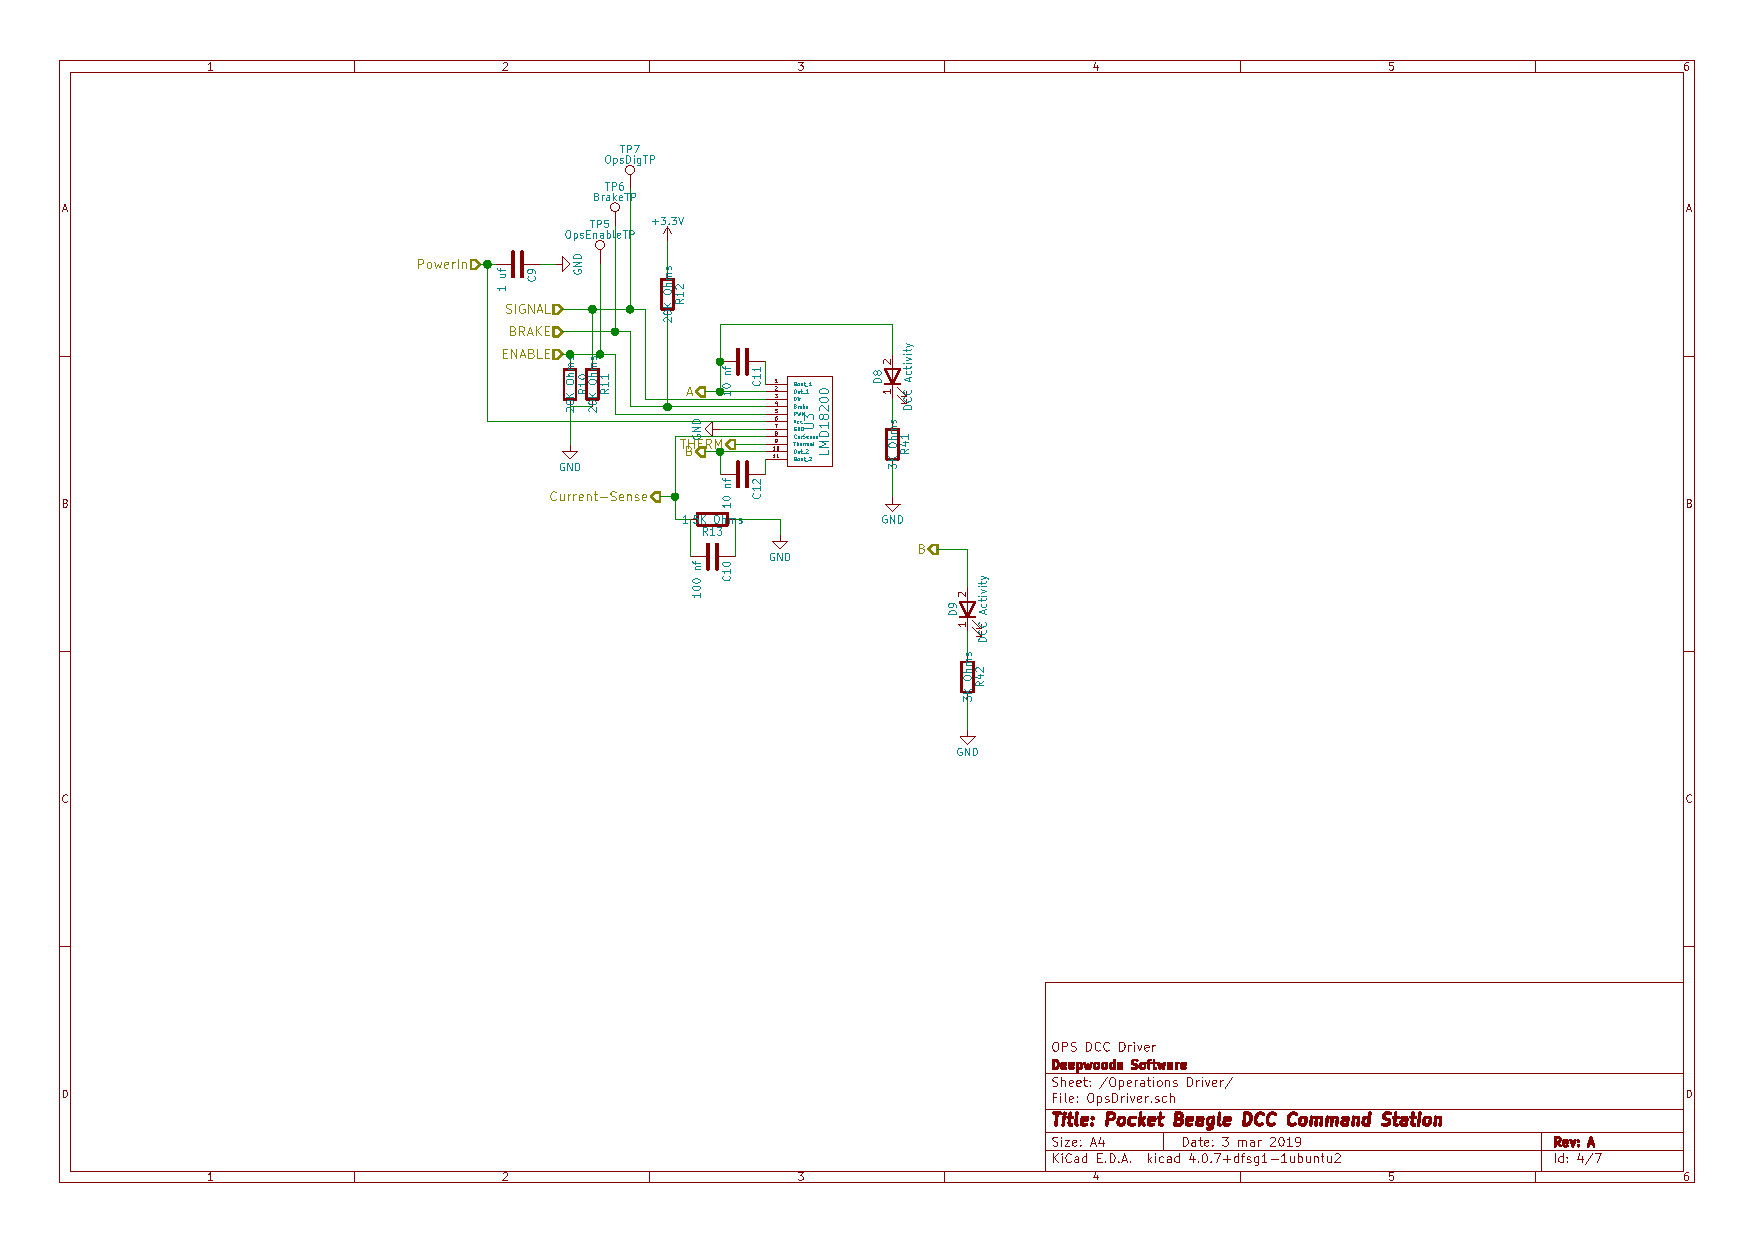
\includegraphics[width=4in]{PocketBeagleCommandStation-4.pdf}
\caption{Circuit Diagram of the PocketBeagleCommandStation board, page 4: OPS 
DCC Driver}
\end{centering}\end{figure}

This shows the OPS DCC Driver circuitry.
\clearpage
\subsection{Programming and Alt drivers}
\begin{figure}[hbpt]\begin{centering}%
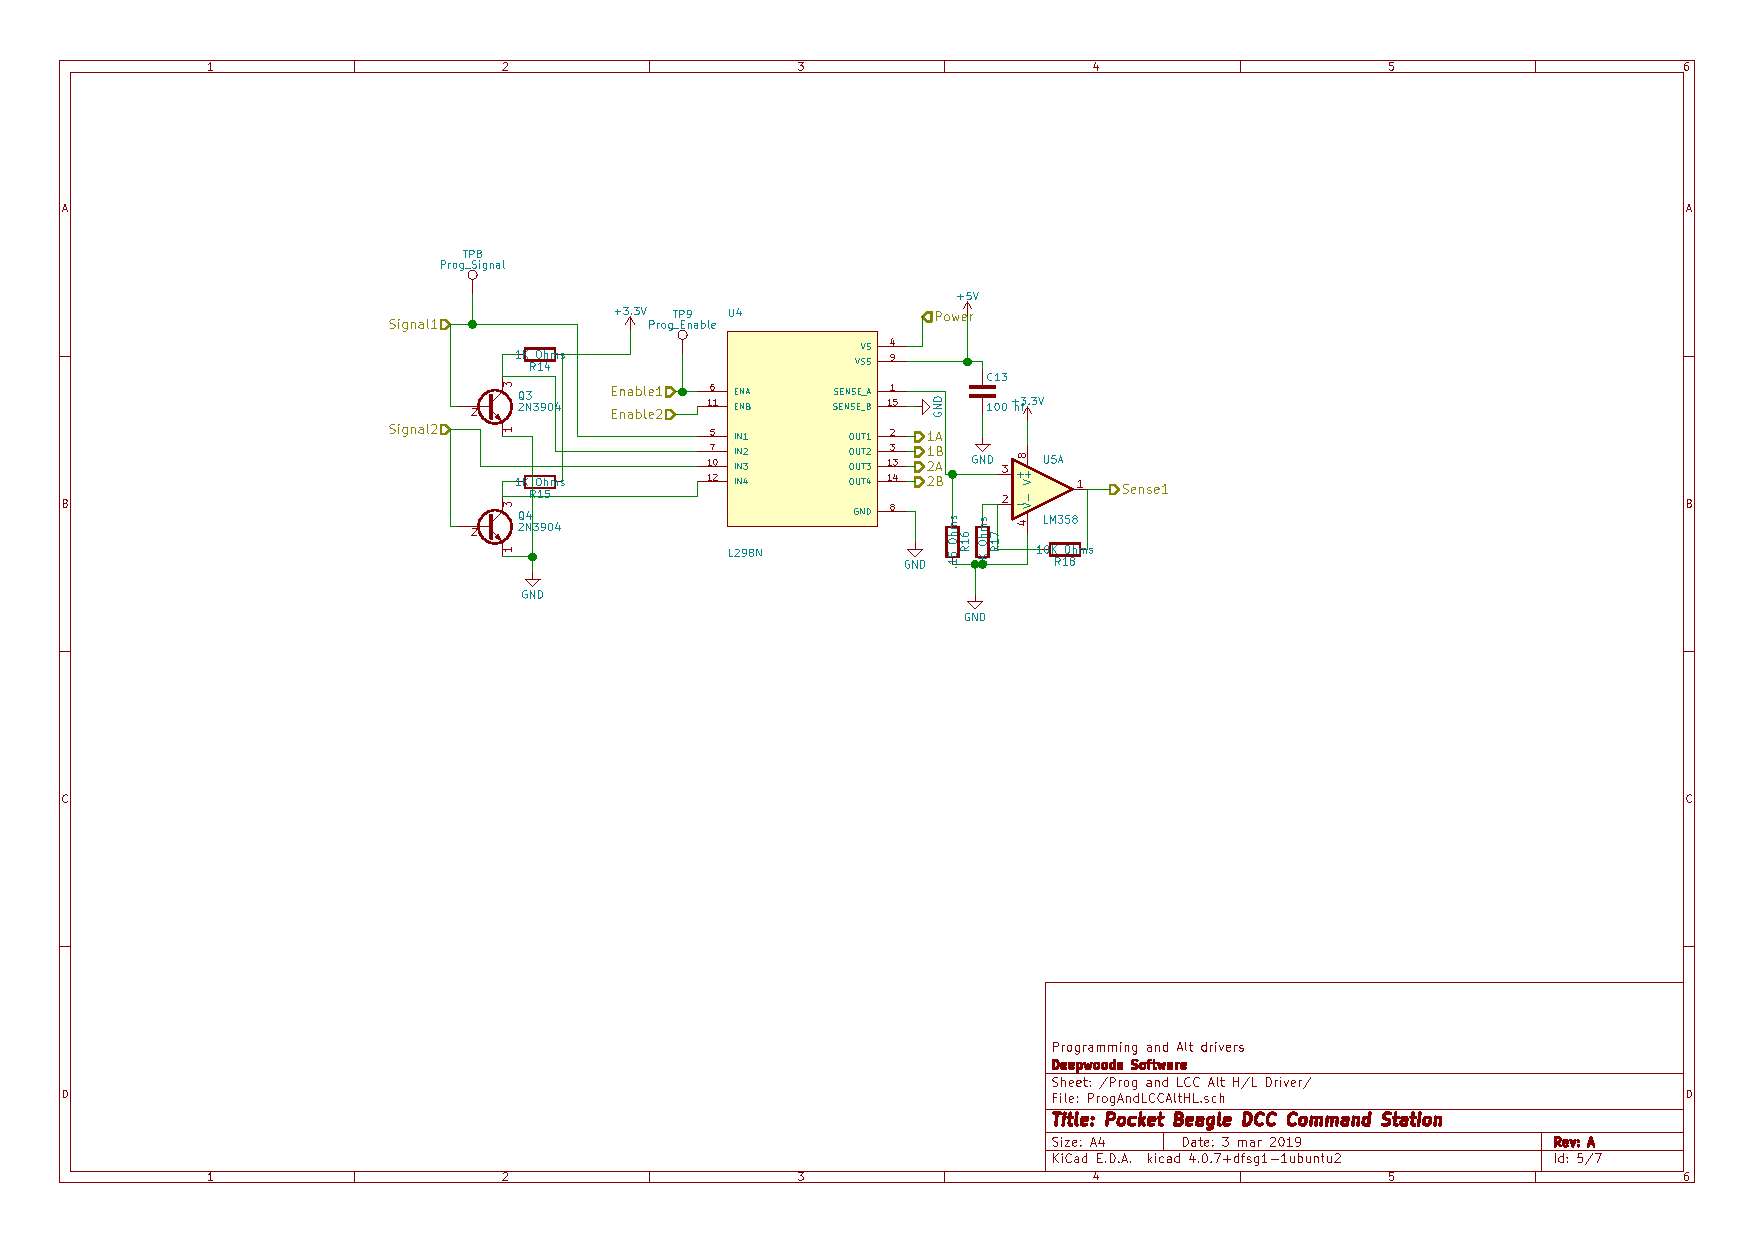
\includegraphics[width=4in]{PocketBeagleCommandStation-5.pdf}
\caption{Circuit Diagram of the PocketBeagleCommandStation board, page 5: 
Programming and Alt. DCC Driver}
\end{centering}\end{figure}

This shows the Programming and Alt. DCC Driver circuitry.
\clearpage
\subsection{Railcom Interface}
\begin{figure}[hbpt]\begin{centering}%
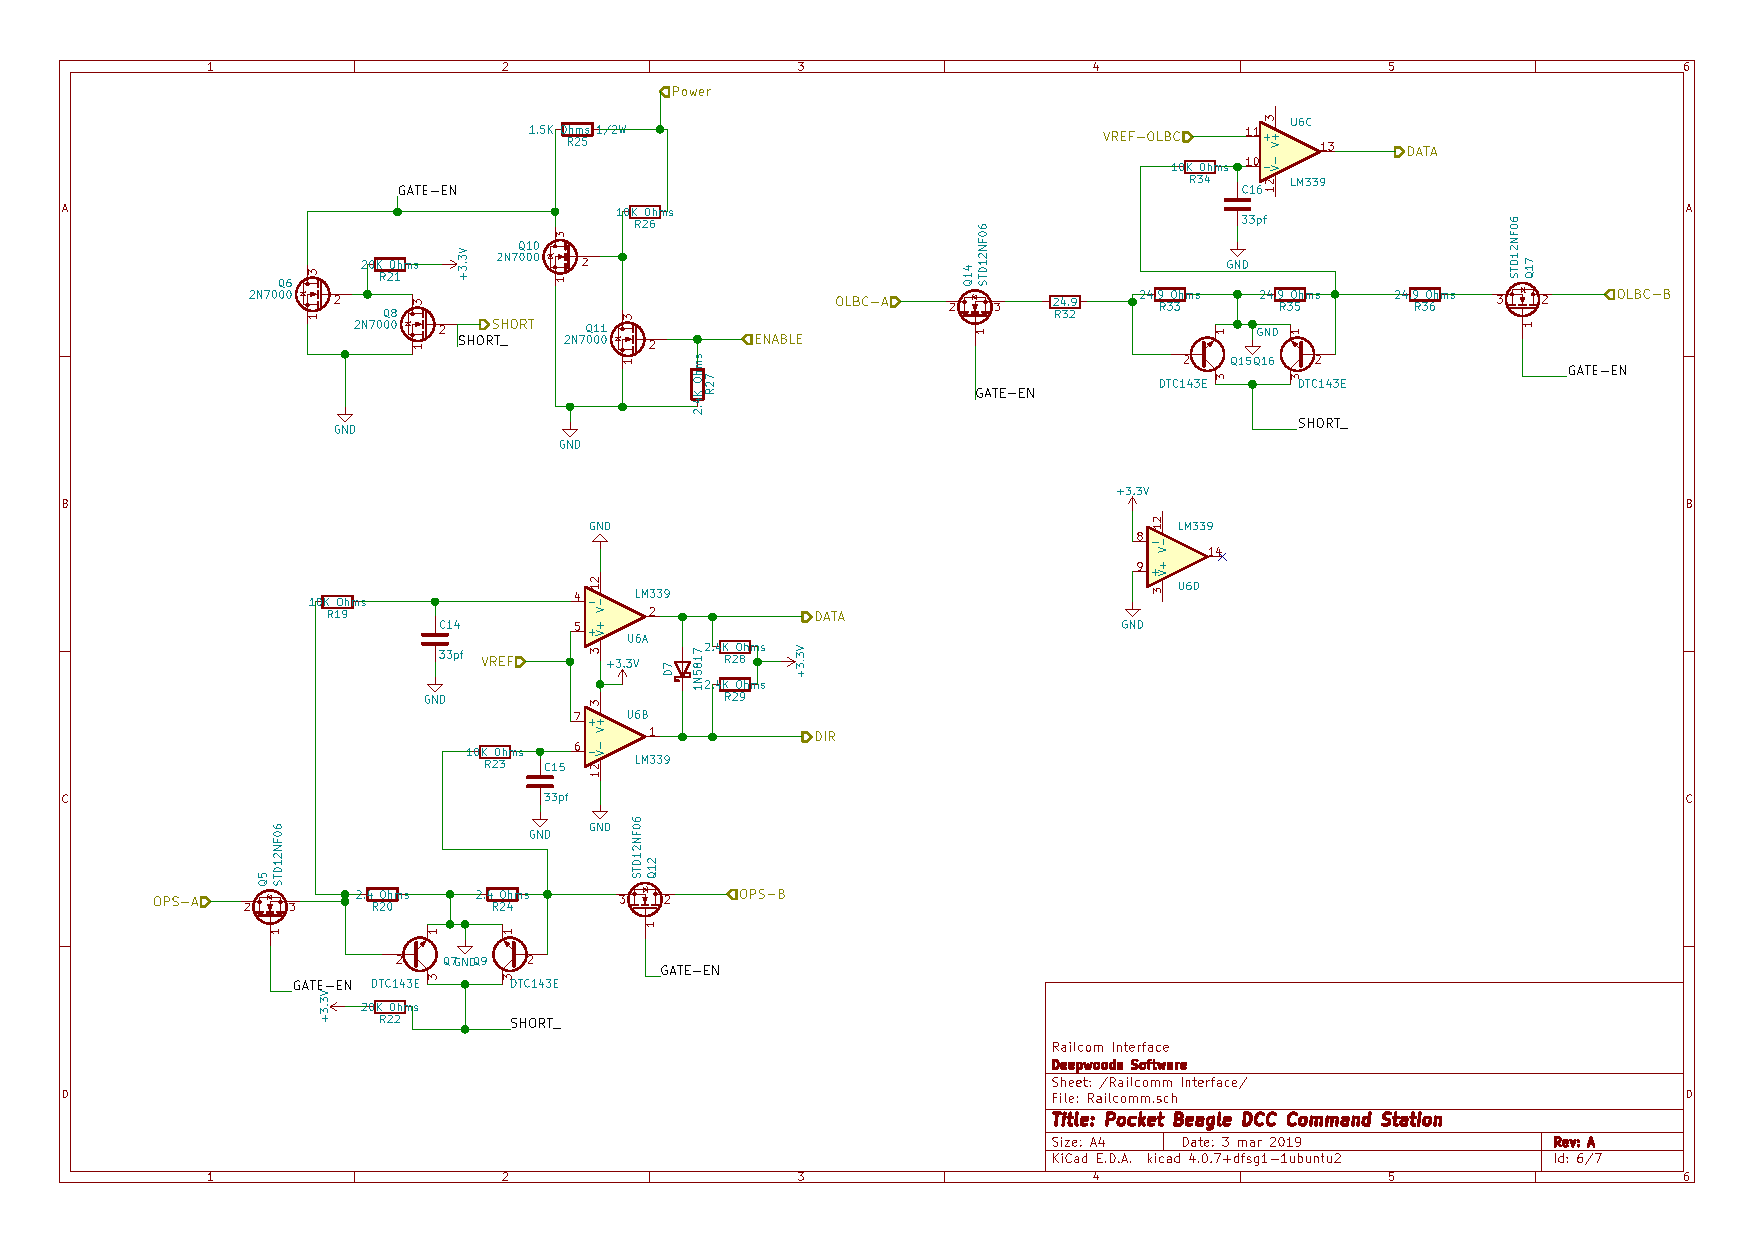
\includegraphics[width=4in]{PocketBeagleCommandStation-6.pdf}
\caption{Circuit Diagram of the PocketBeagleCommandStation board, page 6: 
Railcom Interface}
\end{centering}\end{figure}

This shows the Railcom Interface circuitry.
\clearpage
\subsection{Fan Control}
\begin{figure}[hbpt]\begin{centering}%
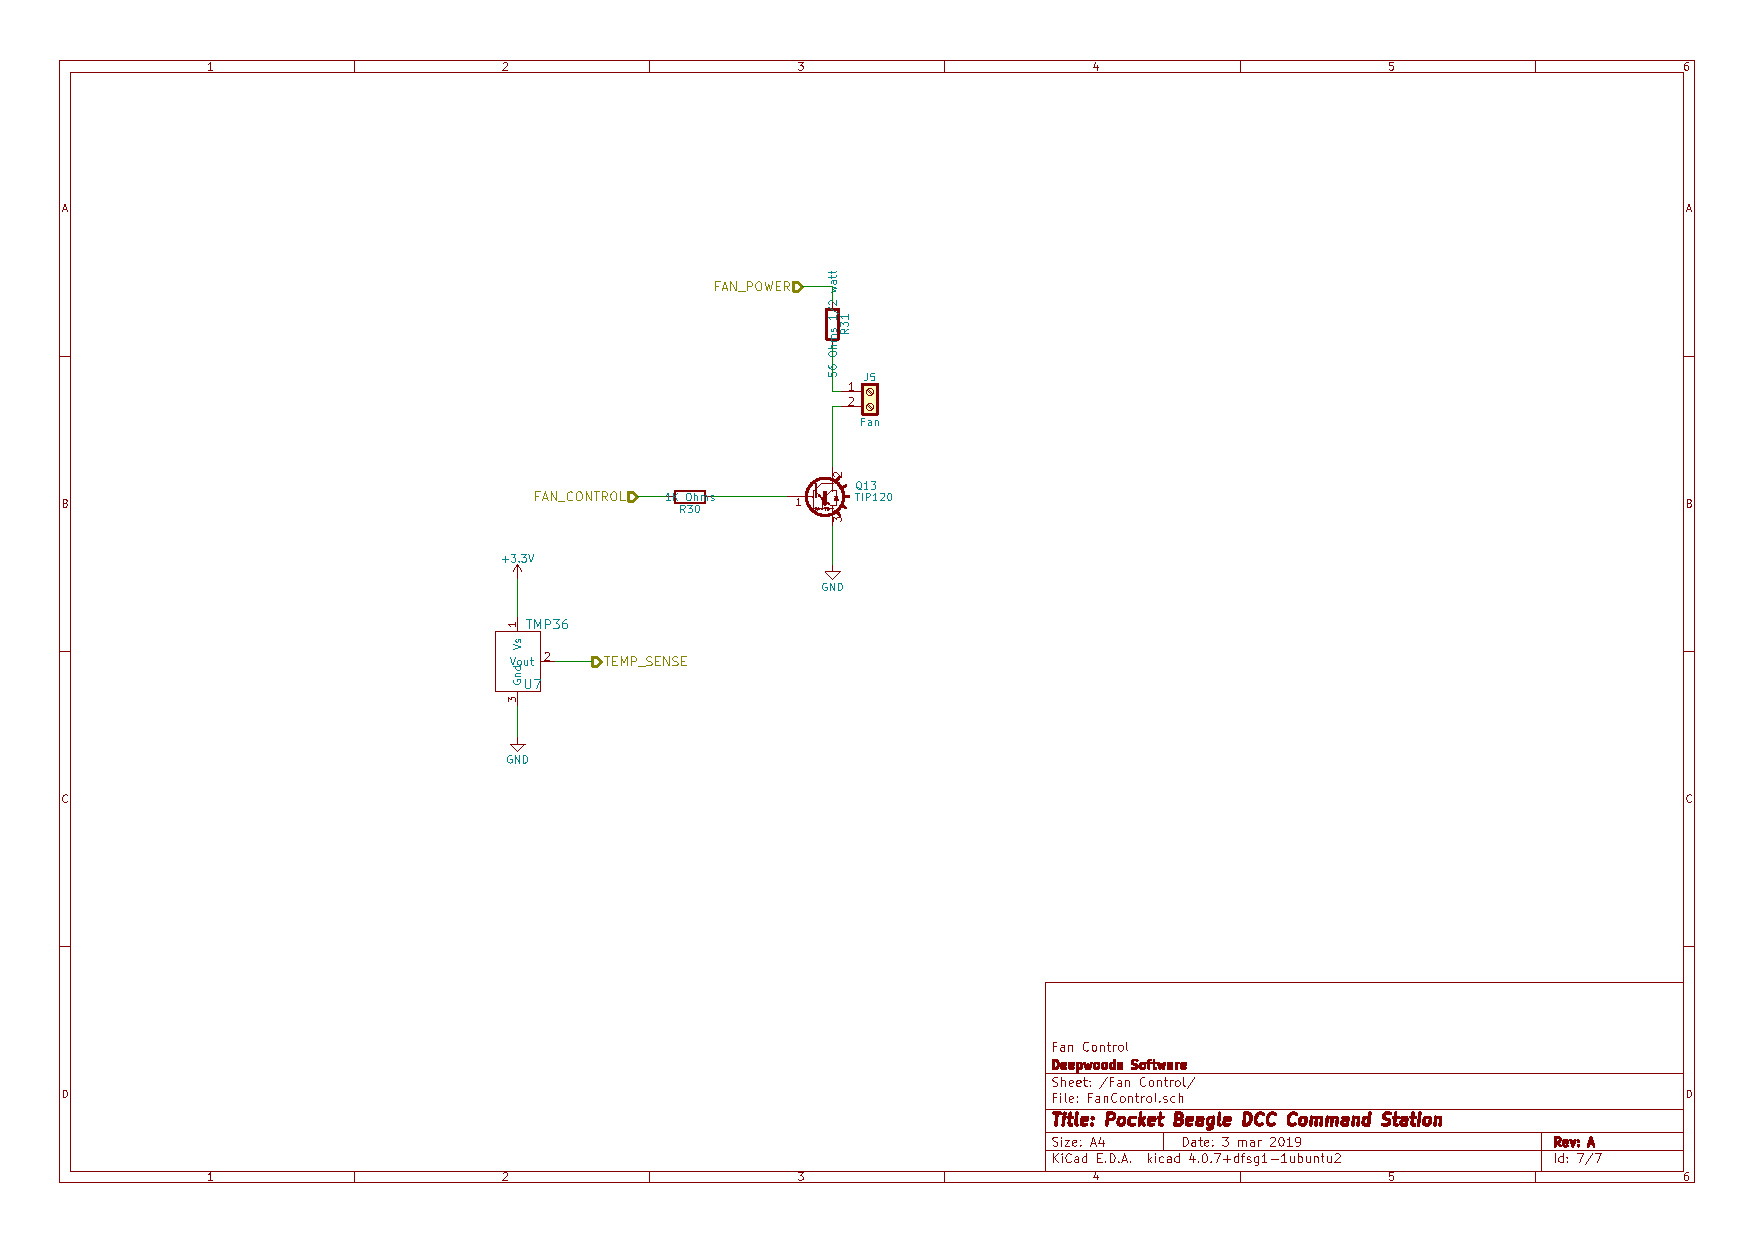
\includegraphics[width=4in]{PocketBeagleCommandStation-7.pdf}
\caption{Circuit Diagram of the PocketBeagleCommandStation board, page 7: 
Fan and temperature control}
\end{centering}\end{figure}

This shows the Fan and temperature control circuitry.
\clearpage
\section{Heatsink and Fan}

\section{General Wiring Notes}

\section{Configuration}




